\documentclass[12pt]{article}

\usepackage{color}
\usepackage{float}
\usepackage{answers}
\usepackage{setspace}
\usepackage{graphicx}
\usepackage{enumitem}
\usepackage{multicol}
\usepackage{mathrsfs}
\usepackage[margin=1in]{geometry} 
\usepackage{amsmath,amsthm,amssymb}
 
\newcommand{\N}{\mathbb{N}}
\newcommand{\Z}{\mathbb{Z}}
\newcommand{\C}{\mathbb{C}}
\newcommand{\R}{\mathbb{R}}

\DeclareMathOperator{\sech}{sech}
\DeclareMathOperator{\csch}{csch}
 
\newenvironment{theorem}[2][Theorem]{\begin{trivlist}
\item[\hskip \labelsep {\bfseries #1}\hskip \labelsep {\bfseries #2.}]}{\end{trivlist}}
\newenvironment{definition}[2][Definition]{\begin{trivlist}
\item[\hskip \labelsep {\bfseries #1}\hskip \labelsep {\bfseries #2.}]}{\end{trivlist}}
\newenvironment{proposition}[2][Proposition]{\begin{trivlist}
\item[\hskip \labelsep {\bfseries #1}\hskip \labelsep {\bfseries #2.}]}{\end{trivlist}}
\newenvironment{lemma}[2][Lemma]{\begin{trivlist}
\item[\hskip \labelsep {\bfseries #1}\hskip \labelsep {\bfseries #2.}]}{\end{trivlist}}
\newenvironment{exercise}[2][Exercise]{\begin{trivlist}
\item[\hskip \labelsep {\bfseries #1}\hskip \labelsep {\bfseries #2.}]}{\end{trivlist}}
\newenvironment{solution}[2][Solution]{\begin{trivlist}
\item[\hskip \labelsep {\bfseries #1}]}{\end{trivlist}}
\newenvironment{problem}[2][Problem]{\begin{trivlist}
\item[\hskip \labelsep {\bfseries #1}\hskip \labelsep {\bfseries #2.}]}{\end{trivlist}}
\newenvironment{question}[2][Question]{\begin{trivlist}
\item[\hskip \labelsep {\bfseries #1}\hskip \labelsep {\bfseries #2.}]}{\end{trivlist}}
\newenvironment{corollary}[2][Corollary]{\begin{trivlist}
\item[\hskip \labelsep {\bfseries #1}\hskip \labelsep {\bfseries #2.}]}{\end{trivlist}}
 
\begin{document}
% --------------------------------------------------------------
%                         Start here
% --------------------------------------------------------------
 
\title{HW1}%replace with the appropriate homework number
\author{Seyed Armin Vakil Ghahani\\ %replace with your name
PSU ID: 914017982\\
CSE-565 Fall 2018\\
Collaboration with:
Sara Mahdizadeh Shahri, Soheil Khadirsharbiyani,\\
Muhammad Talha Imran} %if necessary, replace with your course title
 
\maketitle
%Below is an example of the problem environment
\begin{problem}{1}
Problem 2, Chapter 1 on page 22 of the Textbook. (Pair ranks each other first)
\end{problem}

%Below is the solution environment
\begin{solution}{}
\textit{True.} Prove by contradiction.
Suppose S is the stable matching that has not $(m,w)$ pair.
$m$ is matched to a woman named $w_1$, and $w$ is matched to a man named $m_1$.
In this matching, $m$ prefers $w$ to $w_1$ because $w$ is ranked first on his preference
list. In addition, $w$ prefers $m$ to $m_1$ because $m$ is also ranked first on her 
preference list. So, this pair is unstable, and it is in contradiction with the
first assumption that S is a stable matching.
\end{solution}



\begin{problem}{2}
Solve Problem 4, Chapter 1 on page 23 of the Textbook. (Hospitals vs Residents)
\end{problem}

%Below is the solution environment
\begin{solution}{}
Assume, hospital $h_i$ wants to hire $x_i$ residents. Make a bipartite graph
which has $\sum_{i=1}^{m} x_i$ vertexes in one part that each vertex represents one
position in the corresponding hospital, and $n$ vertexes in the other part that represents
medical students. Suppose a student $n_i$ that has the following preference list:
$${h_{i_1},h_{i_2},...,h_{i_m}}$$
For the new graph, expand the preference list as follows:
$${h_{i_11},h_{i_12},...,h_{i_1x_{i_1}}},$$
$${h_{i_21},h_{i_22},...,h_{i_2x_{i_2}}},$$
$$...$$
$${h_{i_m1},h_{i_m2},...,h_{i_mx_{i_m}}}$$
Actually, each hospital $h_i$ in the preference list is repeated $x_i$ times.
Moreover, to make the number of vertexes in each part equal, we add additional
\textit{no hospital} vertexes to the hospital part. These new vertexes are also
added to the end of the preference list of each student.

This new stable matching problem can be solved by the Gale-Shapley's algorithm 
with the new stability definition. Men in the Propose-And-Reject algorithm
are hospitals and women are the students. The difference of the new algorithm
with the main algorithm is the stability definition. To proof the correctness
of the new algorithm, we use contradiction. Suppose $(H,S)$ is an unstable pair in
the graph. There are two cases:
\begin{itemize}
\item $H$ never proposed to $S$.

If $S$ is currently hired by hospital $H$ but assign to the other vertex of this
hospital, this pair is not an unstable pair by definition, and it is in contradiction
with the assumption.

\item $H$ proposed to $S$.

In this case, $S$ rejected $H$ right away or later. So, $S$ prefers his/her assigned 
hospital to $H$. As a result, this pair is stable and contradicts the assumption.
\end{itemize}

\end{solution}



\begin{problem}{3}
Solve Problem 5, Chapter 1 on page 24 of the Textbook. (Stable matchings with indifferences)
\end{problem}

%Below is the solution environment
\begin{solution}{}
\begin{itemize}
\item a. \textit{Yes.} 
In this problem, we change the preferences list of people in this way: In every preference list that
has a tie between two or more people, make the preference between these people randomly to make the
preference lists like the general stable matching problem. We can run the Gale-Shapley algorithm with
this new preferences list and get the stable matching for this problem. However, it needs to prove 
the stability of the Gale-Shapley algorithm solution, because this part just changes.
To prove the stability, we use the contradiction. Suppose $(A,Z)$ is an unstable pair in
the graph. There are two cases:
\begin{itemize}
\item $Z$ never proposed to $A$.
$Z$ prefer his Gale-Shapley partner to $A$, or he equally prefers his partner and $A$.
So, base on the strong instability definition, this pair is stable.

\item $Z$ proposed to $A$.
In this case, $A$ may reject $Z$ or broke up with him after a better proposal.
In both cases, $A$ prefer $Z$ to her Gale-Shapley partner and this pair is stable.
\end{itemize}

Consequently, in both cases the $(A,Z)$ is a stable pair and its a contradiction.

\item b. \textit{No.}
If a weak instability exists in the problem, it may not solve. Figure \ref{fig:mot3} represents 
an example of this instability.
\begin{figure}[h]
 \centering
 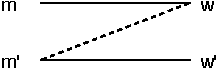
\includegraphics[width=0.50\textwidth]{fig1.pdf}
 \caption{The example of instable matching
 \label{fig:mot3}}
\end{figure}
In this example, $(m,w)$ and $(m',w')$ are the pairs in the matching. $w$ and $w'$ do not prefer
$m$ and $m'$ to each other, and they are both equal for women. However, $m$ and $m'$ are both
prefer $w$ to $w'$. Because of this preference $m'$ and $w$ has weak instability and they want to
broke up with their partners and become together. After this broke up, there is the same situation
for $m$ and $w$, and they have weak instability. This procedure will last forever, and this 
instability will not resolve.

\end{itemize}

\end{solution}



\begin{problem}{4}
Solve Problem 8, Chapter 1 on page 27 of the Textbook. (Truthfulness in stable matchings)
\end{problem}

%Below is the solution environment
\begin{solution}{}
There is an example which a woman can lie about her preferences and match with her
best preference. Table \ref{table:menpref} and \ref{table:truepref} show the correct preferences list of
men and women.

\begin{table}[H]
\centering
\begin{tabular}{ |c|c|c|c| } 
 \hline
 & best & & worst \\
 \hline
 $m$ & $w$ & $w'$ & $w''$ \\ 
 \hline
 $m'$ & $w$ & $w'$ & $w''$ \\ 
 \hline
 $m''$ & $w'$ & $w$ & $w''$ \\ 
 \hline
\end{tabular}
\caption{Preferences of men}
\label{table:menpref}
\end{table}

\begin{table}[h!]
\centering
\begin{tabular}{ |c|c|c|c| } 
 \hline
 & best & & worst \\
 \hline
 $w$ & $m''$ & $m$ & $m'$ \\ 
 \hline
 $w'$ & $m$ & $m''$ & $m'$ \\ 
 \hline
 $w''$ & $m$ & $m''$ & $m'$ \\ 
 \hline
\end{tabular}
\caption{Correct preferences of women}
\label{table:truepref}
\end{table}

\begin{figure}[H]
 \centering
 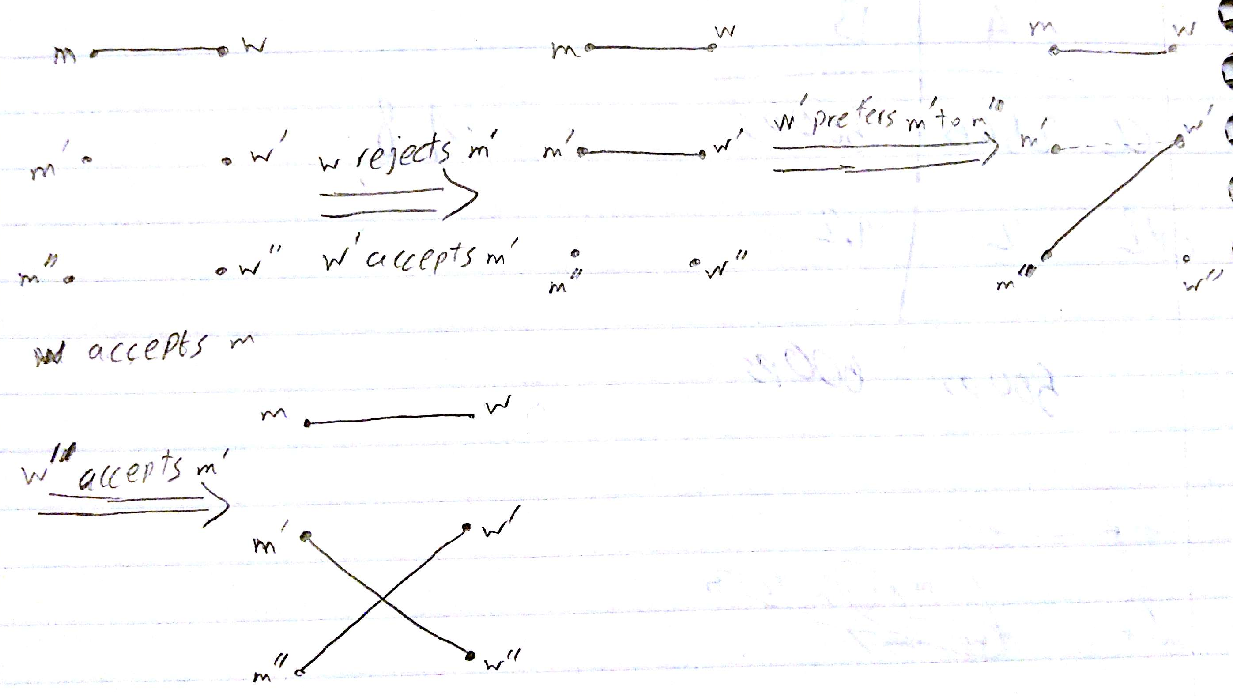
\includegraphics[width=0.50\textwidth]{fig2.pdf}
 \caption{The Gale-Shapley algorithm if women do not lie
 \label{fig:true}}
\end{figure}

Figure \ref{fig:true} shows that $w$ cannot get her best preference if she tells the truth.
However, if she lies about her preferences and women preferences list looks like the \ref{table:falsepref},
the Gale-Shapley algorithm is shown in Figure \ref{fig:wrong}. It is shown that $w$ matches to her
best preference if she lies.

\begin{table}[h!]
\centering
\begin{tabular}{ |c|c|c|c| } 
 \hline
 & best & & worst \\
 \hline
 $w$ & $m''$ & {\color{red} $m'$} & {\color{red} $m$} \\ 
 \hline
 $w'$ & $m$ & $m''$ & $m'$ \\ 
 \hline
 $w''$ & $m$ & $m''$ & $m'$ \\ 
 \hline
\end{tabular}
\caption{Wrong preferences of women}
\label{table:falsepref}
\end{table}

\begin{figure}[H]
 \centering
 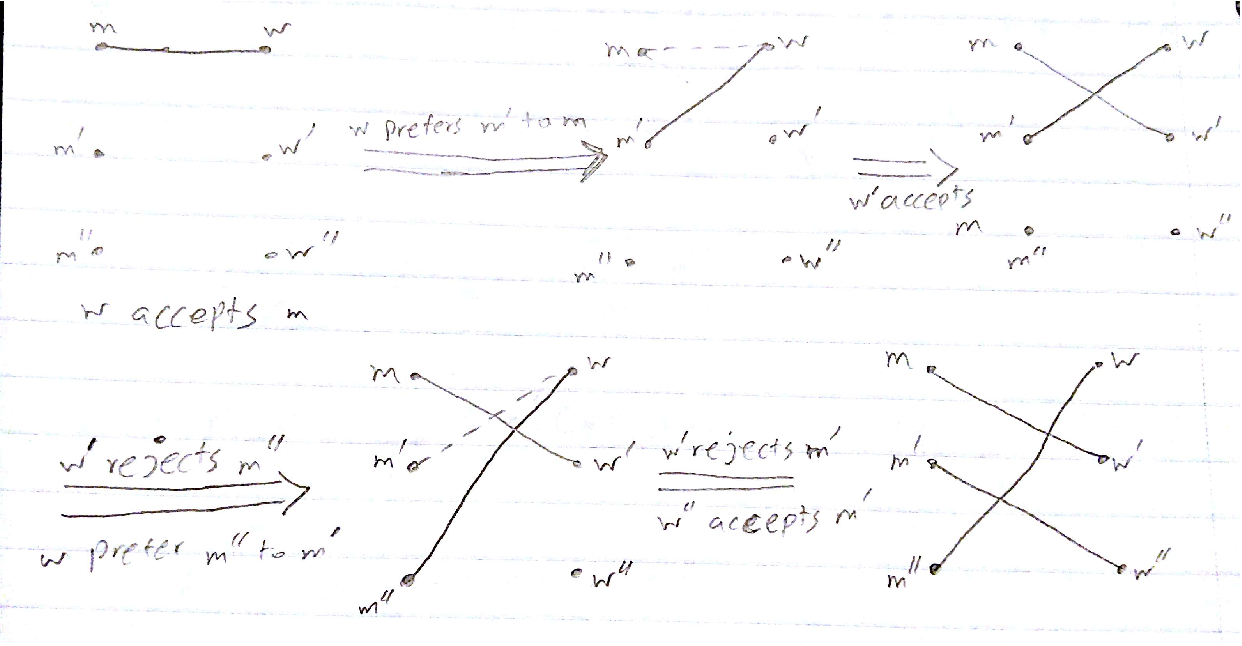
\includegraphics[width=0.50\textwidth]{fig3.pdf}
 \caption{The Gale-Shapley algorithm if women lie
 \label{fig:wrong}}
\end{figure}

\end{solution}

\begin{problem}{5}
Solve Problem 5, Chapter 2 on page 68 of the Textbook. (Implications for O-notation)

The question is whether the statements under (a), (b), (c) are always true for $f(n) \in O(g(n))$.
\end{problem}

%Below is the solution environment
\begin{solution}{}
\begin{itemize}
\item (a) This statement is not correct if $f(n)$ and $g(n)$ are constant.
Suppose $f(n)=c_1$ and $g(n)=1$, which $c_1$ is some constant higher than 1.
The $f(n) \in O(g(n))$ is correct for these functions.
%In addition, we know that $f(n)\in O(g(n))$, which means that $f(n) \leq c*g(n)$. So,
The following should be correct:
$$log_2f(n) \leq c_2*log_2g(n) \Leftrightarrow log_2c_1 \leq c_2*log_21$$
$$\Leftrightarrow log_2c_1 \leq c_2*0 \Leftrightarrow log_2c_1 \leq 0$$
Because of $c_1 > 1$ inequality,  the $log_2c_1 \leq 0$ inequality cannot be correct,
and the statement can not be correct.

\item (b) This statement is also wrong if $f(n) = 2g(n)$, which the $f(n) \in O(g(n))$ equation
is correct for that.
If the statement is correct, the following should be correct:
$$2^{f(n)} \leq c*2^{g(n)} \Leftrightarrow 2^{2g(n)} \leq c*2^{g(n)} \Leftrightarrow 2^{g(n)} \leq c$$
Therefore, if $g(n)$ is not a constant value, for any value of $c$, there is some $N$ which
$2^{g(N)} > c$, and it contradicts the $2^{f(n)} \in O(2^{g(n)})$ equation.

\item (c) This statement is correct for any $f(n), g(n)$.
According to the assumption, $f(n) \leq c * g(n)$ which for any value of $n \geq N$ is true.
Therefore, if we square this inequality, $f(n)^2 \leq c^2 * g(n)^2$, this equation is also true
for each $n \geq N$. To prove $f(n)^2 \in O(g(n)^2)$, the constant value is $c^2$, and $n_0$ is $N$.

\end{itemize}
\end{solution}


\pagebreak

\end{document}

